\subsection{Lightcurve}\label{ssec:lightcurve}

Time series data and their analyses are a fundamental part of solar
physics for which many data sources are available.
SunPy provides a \texttt{LightCurve} class
with a convenient and consistent interface for handling solar time-series
data.  The main engine behind the \texttt{LightCurve} class is
the {\texttt{pandas}} data-analysis library.  
\texttt{LightCurve}'s \texttt{data} attribute is a \texttt{pandas.DataFrame} 
object. The \texttt{pandas} library contains a large amount
of functionality for manipulating and analysing time-series data,
making it an ideal basis for \texttt{LightCurve} \citep{mckinney2012}.  \texttt{LightCurve}
assumes that the input data are time-ordered list(s) of numbers, and each
list becomes a column in the \texttt{pandas} DataFrame object.

Currently, the \texttt{LightCurve} class is compatible with the
following data sources: the \textit{GOES} X-ray Sensor (XRS), \textit{PROBA2}/LYRA, and \textit{SDO}/EVE\footnote{Note that only the level ``OCS'' and
average CSV files is currently implemented -- see \url{http://lasp.colorado.edu/home/eve/data/}}.  For each of these instruments, a subclass of the
\texttt{LightCurve} object is initialised
(e.g., \texttt{GOESLightCurve}) which inherits from
\texttt{LightCurve}, but allows instrument-specific functionality to be
included.  Future developments will introduce support for additional
instruments and data products, as well as implementing a factory interface 
similar to that of \texttt{Map}.  Since there is no established standard
as to how time-series data should be stored and distributed, each SunPy 
\texttt{LightCurve} object subclass provides the ability to download its corresponding 
specific data format in its constructor and parse that file type.

A \texttt{LightCurve} object may be created using a number of different methods. 
For example, a \texttt{LightCurve} may be created for a specific instrument given
an input time range. In Listing~\ref{code:goes_lc}, 
the \texttt{LightCurve} constructor searches a remote source for the GOES X-ray 
data specified by the time interval, downloads the required files, and 
subsequently creates and plots the object. Alternatively, if the data file 
already exists on the local system, the \texttt{LightCurve} object may be 
initialised using that file as input.

\begin{listing}[H]
\pythoncode{lightcurve.py}
\begin{center}
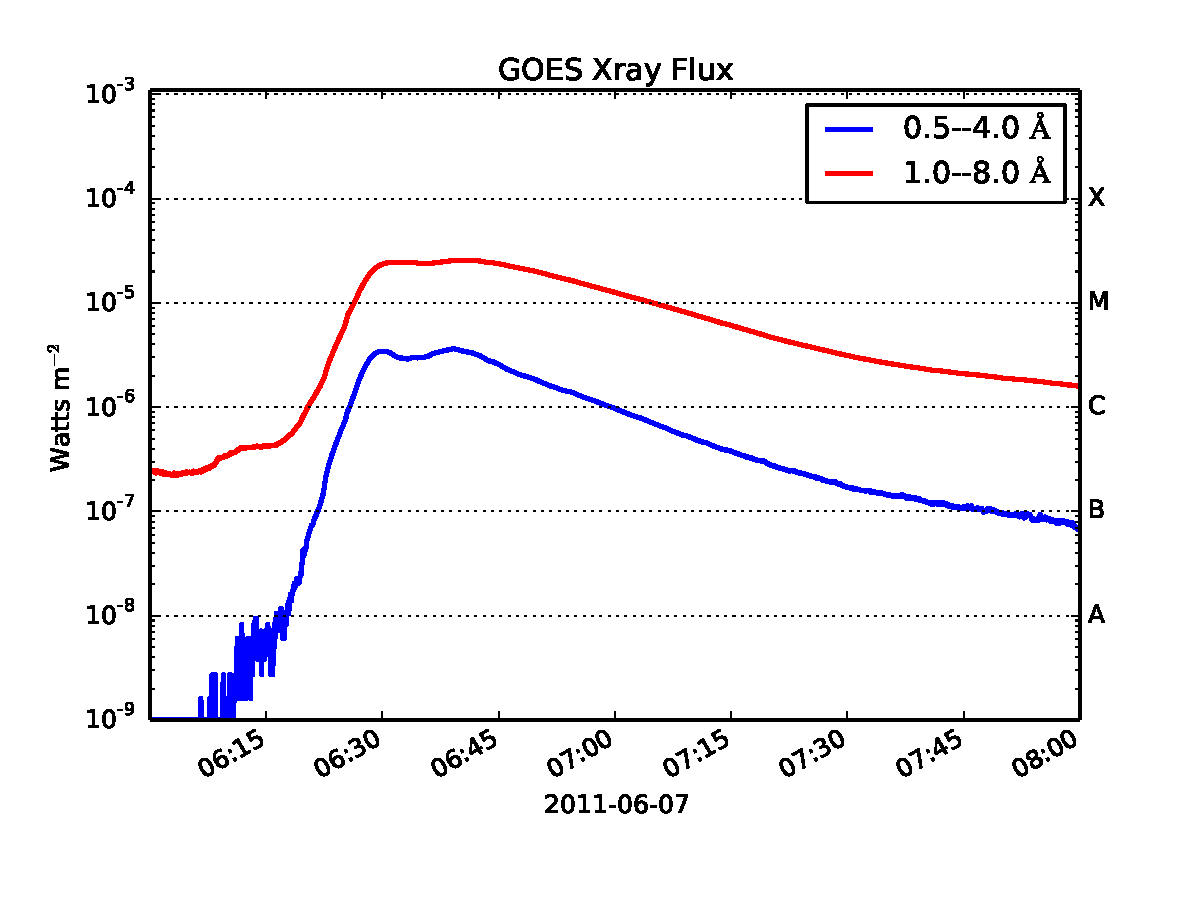
\includegraphics[width=10cm]{goes_lightcurve.pdf}
\end{center}
\caption{Example retrieval of a GOES lightcurve
using a time range and the output of the 
\texttt{peek()} method. The maximum flux value in the \textit{GOES} 1.0--8.0$\AA$\ channel 
is then retrieved along with the location in time of the maximum.}
\label{code:goes_lc}
\end{listing}